
% MISSING PER THE GUIDE (needs new writing by you, not copy-paste):
%   - §3.6: a 3-5 line chapter-opening paragraph for this new Chapter 2
%     (guide says Ch.1 already has a usable opener; this one does not, since
%     the old Ch_3_pca.tex opener was written to introduce PCA specifically,
%     not the whole theory chapter — I left the old PCA-specific opening
%     text in place under §2.1 below rather than inventing a new one).
%============================================================================

\chapter{Machine learning theory}
\label{ch:ml_theory}

\section{Fundamentals of machine learning}
\label{sec:introduction_to_ml}

Machine Learning is the science (and art) of programming computers so they can
learn from data \cite{geron2022hands}.
While classical programming follows fixed, man-defined rules, a machine learning program consists of a function that takes inputs and produces an output based on rules deduced by the algorithm itself, rather than defined by the programmer. 

The examples that the system uses to learn are called \textit{training sets} and are described by numerical features. When a task is presented, the algorithm uses these examples to identify trends beyond what simple statistical analysis can capture and to build a \textit{model}. The patterns found during the learning stage remain informative when new observations are presented, and for this reason the model can be used to make predictions or analyze new data. More specifically, an algorithm is the set of rules and procedures used to solve a specific problem or perform a particular task, while a model is the output or result of applying an algorithm to a data set.

Most machine learning processes require a large amount of high-quality data that will form the basis of the training process.
Performance is automatically improved by varying a large number of internal parameters and as more data is consumed. 

It is common to distinguish two types of methods, \textit{supervised} and \textit{unsupervised}, based on the information available during training. Each has its own strengths and limitations, and it is important to choose the right approach for the specific task:

\begin{itemize}
    \item \textit{supervised}: the input data are labeled and teach the algorithm what conclusions it should draw. This type of learning first requires a human expert to provide the correct answers and label the data. 
A typical supervised learning task is classification;    

       \item \textit{unsupervised}: the computer learns to identify complex schemes without relying on labeled data. The program groups similar data into clusters, autonomously determined based on its own deductions, in the case of the hierarchical clustering algorithm. Or it could transform the original data into a new set of variables that highlight its internal structure; this process, called feature extraction, is related to dimensionality reduction.
       
\end{itemize}


Machine learning offers computational methods for handling large volumes of data, thereby reducing manual processing and making it a powerful tool for decision support and operational analysis. It is used in many technologies that increase laboratory efficiency and automate repetitive activities. Among these advantages, it also makes it possible to extract insights that could not be identified otherwise.
This approach is well suited to Raman spectroscopy of biological tissues. As discussed in \Cref{ch:introduction}, due to the complexity of biological Raman spectra, it is particularly challenging to reduce the sorting problem to a few manually selected bands. For this reason, we prefer to treat the spectra as numerical objects, as it will be described in \cref{sec:origin-structure}, and to rely on computational approaches.

In this chapter, we will present the theoretical principles underlying \textit{Principal Component Analysis (PCA)} and \textit{Artificial Neural Networks (ANN)}, which will be applied to our specific biological problem.


% CLAUDIO: the last two paragraphs above ("This chapter focuses on..." and
% "In this work, PCA is therefore first used...") were written as the
% closing of a chapter whose ONLY subject was PCA. Now that this section
% is folding into a broader "ML framework" section that also leads into
% dimensionality reduction / ANN theory later in the same chapter, you may
% want to trim/reword these two paragraphs so they don't read as a
% chapter-ending promise about a chapter that no longer exists in this
% form. Left untouched per your instructions — flagging only.

% ---------------------------------------------------------------------
% NEW §2.2 "Dimensionality reduction"
% <- OLD: Ch_3_pca.tex \section{Dimensionality reduction} (same title,
%    unchanged; only the section number changes from old 3.1 to new 2.2).
% ---------------------------------------------------------------------
\section{Dimensionality reduction}
\label{sec:dimensionality_reduction}

The dataset can be represented as a numerical matrix

\begin{equation}
    \mathbf{X} \in \mathbb{R}^{n \times p},
    \label{eq:pca_data_matrix}
\end{equation}

where \(n\) is the number of observations and \(p\) is the number of variables. In this work, each observation is a Raman spectrum and \(p = 483\), as described in \Cref{sec:origin-structure}.

When using machine learning methods, thousands or even millions of features can be involved for
each training instance and working directly with all the original variables not only drastically slows down the algorithm but also makes it hard to find a good solution to the problem; it might be appropriate to reduce the representation.

The first reason to suggest this type of choice is that, in many cases, nearby variables are linked due to overlapping signals (as in Raman spectra, where spectral bands are broad and rich in correspondence). Hence, the \(p\) variables do not necessarily represent \(p\) independent sources of information. Dimensionality reduction replaces the original variables with a smaller and new set of components that retain the dataset's main structure.

The motivation for this step is also connected to the so-called \textit{curse of dimensionality} \cite{geron2022hands}. Each observation can be seen not only as a curve or signal but also as a point in a \(p\)-dimensional space. 
In low-dimensional spaces, points can be relatively close to one another, but when the number of variables increases, distances and volumes grow exponentially with it. High-dimensional data are prone to sparsity, and maintaining the same density of training instances would require an exponentially larger number of observations. For example, with just \(100\) features, you would need more training instances than atoms in the observable universe in order for training instances to be within \(0{,}1\) of each other on average, assuming they were spread out uniformly across all dimensions \cite{geron2022hands}. 
This leads to important consequences for a learning algorithm, because it also means that a new instance
will likely be far away from any training instance, making predictions much less reliable than in lower dimensions.
The more dimensions the training set has, the greater the risk of overfitting it.

Although it will speed up training, reducing dimensionality does lose some information; thus, it cannot be said to automatically lead to an improvement. Its effect must be evaluated in terms of downstream classification performance.


% ---------------------------------------------------------------------
% NEW §2.3 "Principal Component Analysis"
% <- OLD: Ch_3_pca.tex \section{Principal Component Analysis} (same
%    title; old 3.2 -> new 2.3).
% ---------------------------------------------------------------------
\section{Principal Component Analysis}
\label{sec:pca_theory}

In most real-world problems, training instances are not spread out uniformly across
all dimensions, but while many features are almost constant, others are highly correlated.

Among the alternatives adopted to pursue dimensionality reduction are projection-based methods, in which the original data are represented in a lower-dimensional subspace by projecting each observation onto a new set of axes. If the data lie close to a much lower-dimensional subspace, this projection can preserve much of the relevant structure while using fewer coordinates. 

PCA is an \textit{unsupervised} machine learning algorithm commonly used to identify the axis that accounts for the largest amount of variance in the training set. First it identifies the hyperplane that lies closest to the data, and then
it projects the data onto it. 
The procedure builds a new set of orthogonal directions, called \textit{principal components}, as linear combinations of the original ones. The new set is ordered in the sense that the first component is the direction along which the data vary the most, the second expresses the highest  remaining variance under the condition of orthogonality relative to the first, and with the same criteria, the subsequent ones are computed. The last component is the least representative in terms of variance. Once these new variables have been calculated, the size of the representation can be reduced by keeping only the first main components and neglecting the last, less significant ones.


\subsection{Data centering}
\label{subsec:pca_centering_covariance}

Let \(\mathbf{X} \in \mathbb{R}^{n \times p}\) be the data matrix, where each row \(\mathbf{x}_i^{\mathrm{T}}\) is one observation and each column is one of the \(p\) variables. PCA assumes that the dataset is centered around the origin. The mean vector is computed as

\begin{equation}
    \bar{\mathbf{x}} =
    \frac{1}{n}\sum_{i=1}^{n}\mathbf{x}_i,
    \label{eq:pca_mean_spectrum}
\end{equation}
 and the centered data matrix is
\begin{equation}
    \mathbf{X}_c =
    \mathbf{X} - \mathbf{1}\bar{\mathbf{x}}^{\mathrm{T}},
    \label{eq:pca_centered_matrix}
\end{equation}

where \(\mathbf{1}\) is a column vector of ones. Centering the data means subtracting the average vector from each observation, so that the variations are described around an average profile and not at an absolute level.

% -----------------------------------------------------------------
% NEW §2.3.2 "Principal directions and Singular Value Decomposition"
%        the condensed covariance formulation has been inserted.
%        to be eventually discarded.
% -----------------------------------------------------------------
\subsection{Singular Value Decomposition}
\label{subsec:pca_svd}

The \textit{principal directions} can be obtained through the Singular Value Decomposition (SVD) \cite{brunton2019datadriven} of the centered data matrix. The SVD is a standard matrix factorization technique that decomposes \(\mathbf{X}_c\) in:
\begin{equation}
    \mathbf{X}_c =
    \mathbf{U}\boldsymbol{\Sigma}\mathbf{V}^{\mathrm{T}},
    \label{eq:pca_svd}
\end{equation}

where \(\mathbf{U}\) and \(\mathbf{V}\) have orthonormal columns and \(\boldsymbol{\Sigma}\) is diagonal. The matrix \(\mathbf{V}\) contains the principal components \(\mathrm{PC}_j\) that we are looking for:

\begin{equation}
    \mathbf{V} =
    \begin{bmatrix}
    \mathrm{PC}_1 & \mathrm{PC}_2 & \cdots & \mathrm{PC}_p
    \end{bmatrix}
    \in \mathbb{R}^{p \times p}.
    \label{eq:pca_v_matrix}
\end{equation}

The columns of \(\mathbf{V}\) contain the \textit{right singular vectors} (or \textit{loading vectors}); each of them specifies how the original variables are weighted into the linear combination to form one principal component.

The diagonal entries of \(\boldsymbol{\Sigma}\) are called singular values:

\begin{equation}
    \boldsymbol{\Sigma} =
    \begin{bmatrix}
    \sigma_1 & 0 & \cdots & 0 \\
    0 & \sigma_2 & \cdots & 0 \\
    \vdots & \vdots & \ddots & \vdots \\
    0 & 0 & \cdots & \sigma_p
    \end{bmatrix}
    \in \mathbb{R}^{p \times p}.
    \label{eq:pca_sigma_matrix}
\end{equation}

The singular values express the importance of the corresponding main component in describing the variability of the observations and are ordered from the largest to the smallest, arranging the components according to a hierarchy.

The columns of \(\mathbf{U}\) are the corresponding \textit{left singular vectors}, which provide normalized coordinates of the spectra along these directions:

\begin{equation}
    \mathbf{U} =
    \begin{bmatrix}
    \mathbf{u}_1 & \mathbf{u}_2 & \cdots & \mathbf{u}_p
    \end{bmatrix}
    \in \mathbb{R}^{n \times p}.
    \label{eq:pca_u_matrix}
\end{equation}

When these coordinates are scaled by the singular values in \(\boldsymbol{\Sigma}\), they give the projection of the original instances onto the principal components. These projected coordinates are called \textit{scores}.

Let \(\mathbf{W}_d\) be the matrix containing the first \(d\) columns of \(\mathbf{V}\). For \(d\) retained principal components, the matrix that represents the projection of the dataset into the new subspace is written as

\begin{equation}
    \mathbf{X}_{d\text{-proj}} =
    \mathbf{X}_c \mathbf{W}_d =
    \mathbf{U}_d\boldsymbol{\Sigma}_d,
    \label{eq:pca_scores_svd}
\end{equation}

where \(\mathbf{X}_{d\text{-proj}} \in \mathbb{R}^{n \times d}\). 

The principle underlying dimensionality reduction is summarized in the following rank-\(d\) approximation:

\begin{equation}
    \mathbf{X}_c \approx
    \mathbf{U}_d\boldsymbol{\Sigma}_d\mathbf{W}_d^{\mathrm{T}}.
    \label{eq:pca_low_rank}
\end{equation}

In this way, the original dataset was reconstructed using a smaller number \(d\) of directions instead of all the initial \(p\) variables. 
Instead of arbitrarily choosing the number of dimensions to reduce down to, it is
generally preferable to choose the number that adds up to a sufficiently
large portion of the variance (e.g., \(95\%\)).
The metrics analyzed in order to make this assessment are the \textit{Explained Variance Ratio} (EVR), which reveals the variance fraction explained by each \(\mathrm{PC}_j\) component, strictly linked to the singular values as shown in the formula

\begin{equation}
    \mathrm{EVR}_j =
    \frac{\sigma_j^2}{\sum_{k=1}^{p}\sigma_k^2}
    \label{eq:pca_explained_variance_ratio_svd},
\end{equation}

and for a global view, the \textit{Cumulative Explained Variance} (CEV), meaning the progressive sum of the \(\mathrm{EVR}_j\) up to the \(d\)-th component

\begin{equation}
    \mathrm{CEV}_d =
    \sum_{j=1}^{d}\mathrm{EVR}_j =
    \frac{\sum_{j=1}^{d}\sigma_j^2}{\sum_{k=1}^{p}\sigma_k^2}.
    \label{eq:pca_cumulative_explained_variance_svd}
\end{equation}

Both range between \(0\) and \(1\) and can be expressed as percentages. 




\section{Artificial Neural Networks}
\label{sec:ann_fundamentals}

To introduce artificial neural networks (ANN) \cite{Goodfellow-et-al-2016}, it is useful to understand first linear models and see how to overcome their limitations. Linear models, such as linear regression, can fit data efficiently and reliably. The problem with linear models is that their fitting capacity is limited to linear functions.

Artificial neural networks, on the contrary, are able to approximate any function. More precisely, the \textbf{Universal Approximation Theorem} \cite{prince2023understanding} states that there exists a network with one hidden layer containing a finite number of hidden units that can approximate any specified continuous function on a compact subset of $\mathbb{R}^n$ to arbitrary accuracy. This was proved by Cybenko (1989) for a class of sigmoid activations and was later shown to be true for a larger class of nonlinear activation functions. The terms used in the theorem will be explained in the following sections.


\subsection{Neurons, weights and bias}
\label{subsec:neurons}

Artificial neural networks owe their name to the loose analogy between artificial neurons and biological neurons.
Biological neurons \cite{geron2022hands} are composed of a cell body with multiple ramifications. The main branch is called the axon, and it connects to other neurons through synapses. Biological neurons receive short electrical impulses called signals from other neurons via these synapses. When a neuron receives a sufficient number of signals from other neurons within a few milliseconds, it fires its own signals. Individual biological neurons seem to behave in a simple way, but they are organized in a vast network, often in consecutive layers, with each neuron typically connected to thousands of other neurons.

A simple model for the behavior of biological neurons, the artificial neuron, has one or more binary (on/off) inputs and one binary output. The artificial neuron simply activates its output when more than a certain number of its inputs are active.

The Perceptron is a slightly more refined model, based on a linear threshold unit (LTU): the inputs and output are now numbers (instead of binary on/off values) and each input connection is associated with a weight. The LTU computes a weighted sum of its inputs:

\begin{equation}
    z = w_1 x_1 + w_2 x_2 + \cdots + w_n x_n = x^T w
\end{equation}

It then applies a step function to that sum and outputs the result:

\begin{equation}
h_w(x) = \text{step}(z)
\end{equation}

A Perceptron is simply composed of a single layer of TLUs, with each TLU connected to all the inputs. When all the neurons in a layer are connected to every neuron in the previous layer (its input neurons), it is called a \textit{dense layer}.

\begin{figure}[ht]
    \centering
    \subfloat[Single Perceptron: inputs are combined via a weighted sum then passed through a step function.\label{fig:perceptron}]{
        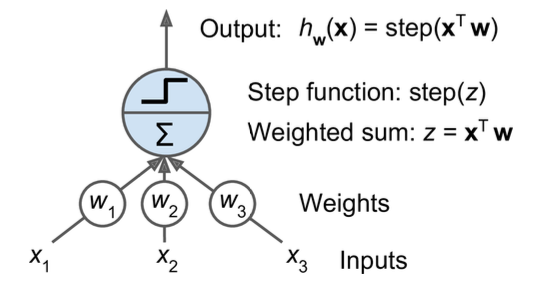
\includegraphics[width=0.47\textwidth]{Images/images_ch_2/perceptron.png}
    }
    \hfill
    \subfloat[Two-layer Perceptron: multiple TLUs stacked into an input and an output layer.\label{fig:two_layer_perceptron}]{
        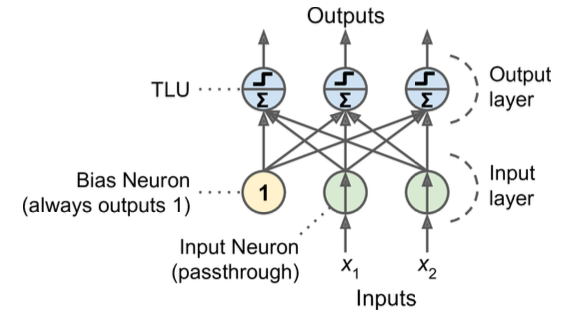
\includegraphics[width=0.47\textwidth]{Images/images_ch_2/two_layer_perceptron.png}
    }
    \caption{Perceptron architectures~\cite{geron2022hands}.}
    \label{fig:perceptrons}
\end{figure}

Moreover, an extra input called \textit{bias} is added ($x_0 = 1$): it is typically represented using a special type of neuron called a bias neuron, which just outputs 1 all the time. The bias shifts the activation boundary away from the origin.


\subsection{Forward propagation and backpropagation}
\label{subsec:forward_back}

The outputs of a layer of artificial neurons for several instances at once can be expressed through the following equation:

\begin{equation}
h_{\mathbf{W, b}}(\mathbf{X}) = \phi (\mathbf{X W} + \mathbf{b})
\end{equation}

\begin{itemize}
    \item As always, $\mathbf{X}$ represents the matrix of input features. It has one row per instance (e.g. spectrum), one column per feature (e.g. principal component).
    \item The weight matrix $\mathbf{W}$ contains all the connection weights except for the ones from the bias neuron. It has one row per input neuron, for the first layer it corresponds to the number of features, and one column per artificial neuron in the layer.
    \item The bias vector $\mathbf{b}$ contains all the connection weights between the bias neuron and the artificial neurons. It has one bias term per artificial neuron.
    \item The function $\phi$ is the activation function (e.g. step, sigmoid or ReLU).
\end{itemize}

Initially, perceptrons were trained by accounting for the error made by the network on a single training instance at a time. The weights of connections that helped reduce the error between prediction and ground truth were reinforced:

\begin{equation}
    w_{i,j}^{(\text{new})} = w_{i,j} + \eta \left( y_j - \hat{y}_j \right) x_i
    \label{eq:perceptron_update}
\end{equation}

where $x_i$ is the $i$-th input value of the current training instance, $\hat{y}_j$ is the predicted output of the $j$-th neuron, $y_j$ is the target output, and $\eta$ is the learning rate.
This learning method, solely based on the prediction for one instance, cannot be applied in networks with more than one hidden layer. This is due to not being able to isolate the role of a single connection in the prediction. The method, however, strongly resembles gradient descent.

In the case of networks with more than one hidden layer, called \textit{deep neural networks} (DNN), weights are updated through the \textit{backpropagation} algorithm, which is based on gradient descent. In two passes through the network (one forward, one backward), the backpropagation algorithm computes the gradient of the network's error with respect to every single model parameter:

\begin{enumerate}
    \item It takes one mini-batch at a time (for example containing 32 instances each), and it goes through the full training set multiple times. Each pass is called an \textit{epoch}.
    \item The output for every instance in the mini-batch is computed layer by layer. This is the \textit{forward pass}: it is like making predictions, but all intermediate results are preserved since they are needed for the backward pass.
    \item The algorithm measures the network's output error through a chosen loss function.
    \item It computes how much each connection in a layer contributed to the error. This is done analytically by applying the chain rule, from the output layer to the first one. This is the \textit{backward pass}.
    \item Finally, the algorithm performs a Gradient Descent step to tweak all the connection weights in the network, using the error gradients it just computed.
\end{enumerate}

More formally, for a network with $D$ layers, the loss is a composition:

\begin{equation}
    \mathcal{L} = L\!\Big(f^{(D)}\big(\cdots f^{(1)}(\mathbf{X};\, \mathbf{W}^{(1)}) \cdots;\, \mathbf{W}^{(D)}\big)\Big)
\end{equation}

where $L(\cdot)$ is the loss function and $f^{(i)}$ the full layer transformation for layer $i$ (i.e. $\phi\!\left(\mathbf{X}\mathbf{W}^{(i)} + \mathbf{b}^{(i)}\right)$).

The goal of backpropagation is to compute $\frac{\partial \mathcal{L}}{\partial \mathbf{W}^{(r)}}$ for every layer $r$, so that each weight matrix can be updated by gradient descent.

For layer $r$, preactivation $\mathbf{z}^{(r)}$ and activation $\mathbf{h}^{(r)}$ are:

\begin{equation}
    \mathbf{z}^{(r)} = \mathbf{h}^{(r-1)} \mathbf{W}^{(r)} + \mathbf{b}^{(r)}, \qquad \mathbf{h}^{(r)} = \phi\!\left(\mathbf{z}^{(r)}\right), \qquad \mathbf{h}^{(0)} = \mathbf{X}
\end{equation}

Applying the chain rule through all layers from $D$ back to $r$:

\begin{equation}
    \frac{\partial \mathcal{L}}{\partial \mathbf{W}^{(r)}} =
    \frac{\partial \mathcal{L}}{\partial \mathbf{h}^{(D)}} \cdot
    \frac{\partial \mathbf{h}^{(D)}}{\partial \mathbf{z}^{(D)}} \cdot
    \frac{\partial \mathbf{z}^{(D)}}{\partial \mathbf{h}^{(D-1)}} \cdot
    \frac{\partial \mathbf{h}^{(D-1)}}{\partial \mathbf{z}^{(D-1)}} \cdots
    \frac{\partial \mathbf{z}^{(r+1)}}{\partial \mathbf{h}^{(r)}} \cdot
    \frac{\partial \mathbf{h}^{(r)}}{\partial \mathbf{z}^{(r)}} \cdot
    \frac{\partial \mathbf{z}^{(r)}}{\partial \mathbf{W}^{(r)}}
      \label{eq:chain_rule}
\end{equation}

where each intermediate factor is

\begin{equation}
    \frac{\partial \mathbf{h}^{(k)}}{\partial \mathbf{z}^{(k)}} = \phi'\!\left(\mathbf{z}^{(k)}\right), \qquad
    \frac{\partial \mathbf{z}^{(k)}}{\partial \mathbf{h}^{(k-1)}} = \mathbf{W}^{(k)}, \qquad
\end{equation}

Finally, the full gradient can be rewritten in short form as follows

\begin{equation}
    \frac{\partial \mathcal{L}}{\partial \mathbf{W}^{(r)}} = \mathbf{h}^{(r-1)\top} \boldsymbol{\delta}^{(r)}
\end{equation}

where $\boldsymbol{\delta}^{(r)}$ is the \textit{backpropagated error signal} at layer $r$, which compresses all the intermediate derivatives in one term and is computed recursively, while $\mathbf{h}^{(r-1)\top}$ comes from the last term in \eqref{eq:chain_rule}.

Once the gradient is available, each weight matrix is updated by a step in the negative gradient direction:

\begin{equation}
    \mathbf{W}^{(r)}_{\text{new}} \leftarrow \mathbf{W}^{(r)} - \eta \, \frac{\partial \mathcal{L}}{\partial \mathbf{W}^{(r)}}
    \label{eq:gd_update}
\end{equation}

where $\eta > 0$ is the \textit{learning rate}, a hyperparameter controlling the step size. The same update applies to the bias vectors $\mathbf{b}^{(r)}$.

It is important to initialize all the hidden layers' connection weights randomly, otherwise all neurons will be identical, hence evolve in the same way. The model would be equivalent to having a single neuron per layer.


\subsection{Activation functions: sigmoid, ReLU}
\label{subsec:activation_functions}

In order for the backpropagation algorithm to work, the activation function must be changed from the step function to one such that its derivative is well-defined and nonzero everywhere, so that the gradient can always be computed and the weights updated effectively.
Furthermore, the activation functions must be non-linear. If they were linear, the transformation obtained by chaining them would be linear too (for example: $f(x)=x+1,\quad g(x)=2x-1 \quad\Rightarrow\quad f(g(x))=(2x-1)+1$). Without some non-linearity between layers, then even a deep stack of layers is equivalent to a single layer.

Multiple choices are possible for the activation function. In the model developed for this thesis, two functions were used: sigmoid and ReLU.

The \textit{sigmoid function} (also known as \textit{the logistic function}) was historically the first replacement for the step function.

\begin{equation}
    \sigma(z) = \frac{1}{1 + e^{-z}}
\end{equation}

It closely represents the firing rates of biological neurons and, due to squashing any input to a value $\in(0,1)$, it can be interpreted as a probability. It is thus particularly suited for the output layer, which is also where it was implemented in our model.

\begin{figure}[ht]
    \centering
    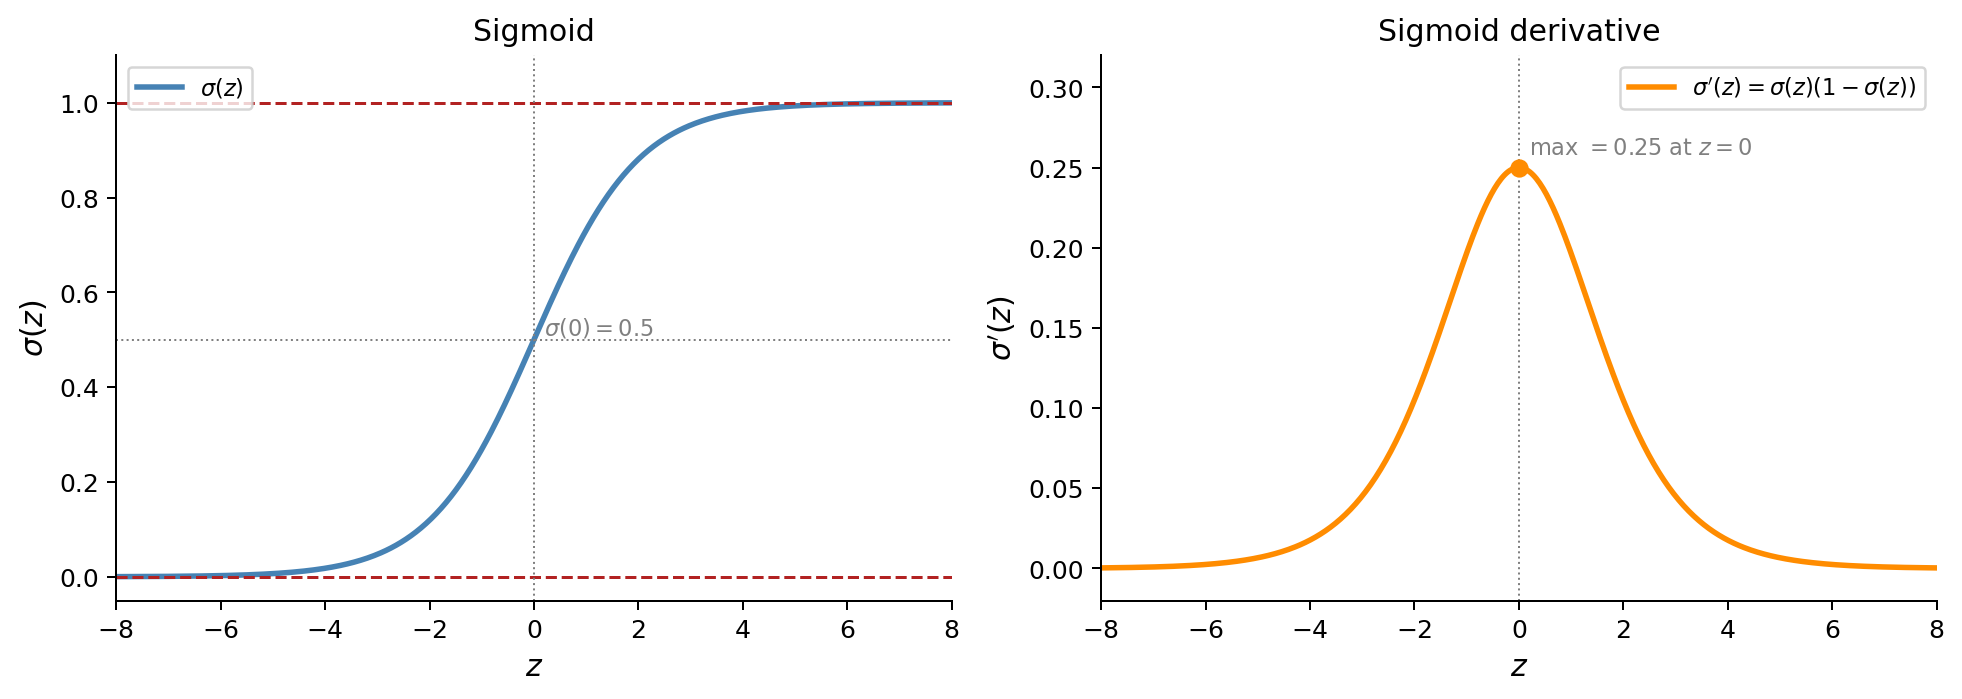
\includegraphics[width=0.9\textwidth]{Images/images_ch_2/sigmoid.png}
    \caption{Sigmoid function $\sigma(z)$ (left) and its derivative $\sigma'(z) = \sigma(z)(1-\sigma(z))$ (right). The shaded regions show the saturation zones where the gradient is nearly zero, slowing down learning through backpropagation.}
    \label{fig:sigmoid}
\end{figure}

The sigmoid shows nevertheless some problems.
Firstly, the saturation of the values of $\sigma(z)$ when $|z|\gg1$ causes the values of the gradient to shrink. Gradients can get progressively smaller as the algorithm progresses
down to the lower layers. As a result, the Gradient Descent update leaves the lower layer connection weights virtually unchanged, and training never converges to a good solution. This is called the \textit{vanishing gradients} problem.
To solve this problem, the hidden layers must have a non-saturating activation function.

The \textit{Rectified Linear Unit} (ReLU) is a simple alternative that doesn't saturate for positive values and has proven to be very effective in deep networks:

\begin{equation}
    \text{ReLU}(z) = \max(0, z)
\end{equation}

It is continuous but not differentiable at z = 0, which can make Gradient Descent bounce around, but it has the advantage of being very fast to compute, significantly reducing training time.
This has been the choice for the hidden layers for the ANN used for this thesis.

\begin{figure}[ht]
    \centering
    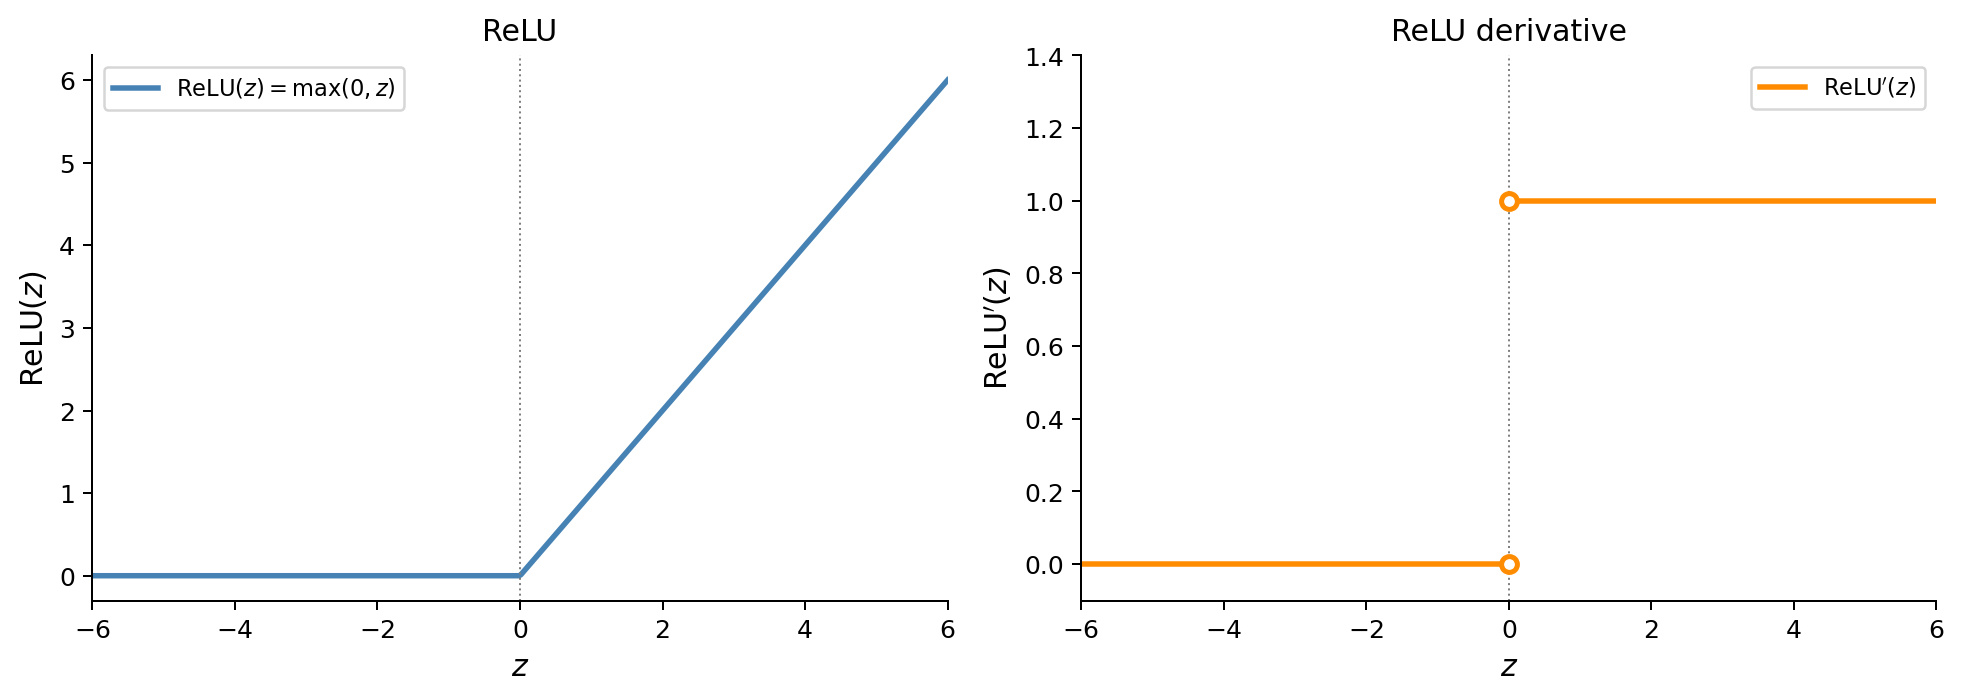
\includegraphics[width=0.9\textwidth]{Images/images_ch_2/relu.png}
    \caption{ReLU function (left) and its derivative (right). For $z < 0$ the output and gradient are both exactly zero (the so-called \textit{dying ReLU} problem), while for $z > 0$ the gradient is a constant 1, avoiding saturation.}
    \label{fig:relu}
\end{figure}

However, ReLU has the disadvantage that its derivative is zero for negative inputs. If all the training examples produce negative inputs to a given ReLU function, the parameters feeding into this ReLU during training cannot be improved, since the gradient with respect to the incoming weights is locally flat. This is known as the \textit{dying ReLU problem}.
To solve it, functions such as LeakyReLU (slightly tilted for $z<0$) exist, but they were not implemented in this work for simplicity.

% -----------------------------------------------------------------
% NEW §2.4.4 "Binary cross-entropy loss"
% <- OLD: Ch_4_ann.tex \subsection{Binary Cross-Entropy Loss} (same
%    title, capitalization style only; old 4.1.4 -> new 2.4.4).
% -----------------------------------------------------------------
\subsection{Binary cross-entropy loss}
\label{subsec:bce}

As seen in the previous sections, Gradient Descent finds the best mapping from input to output by minimizing a \textit{Loss Function}.
Given a dataset $\{(\mathbf{x}_i, y_i)\}$ of input/output pairs, the \textit{loss function}~\cite{prince2023understanding} $L(\boldsymbol{\theta})$ returns a single number that describes the mismatch between the model predictions $f(\mathbf{x}_i, \boldsymbol{\theta})$ and their corresponding ground-truth outputs $y_i$, where $\boldsymbol{\theta}$ denotes the full set of learnable parameters (weights and biases).

Due to the \textit{binary classification} approach discussed in \cref{sec:binary_classification}, the ground-truths for this Artificial neural network will be integers $y_i\in\{0,1\}$. For more complex cases, \textit{multiclass classification}, with $K$ classes and $y_i\in\{0,1,\dots, K-1\}$, can be more useful.

To construct the loss function, a probability distribution based on the output space $y \in \{0,1\}$ must be chosen. A suitable choice is the Bernoulli distribution, which is defined on the domain $\{0,1\}$. This has a single parameter $\lambda \in [0,1]$ that represents the probability that $y$ takes the value one:

\begin{equation}
    \Pr(y|\lambda) = (1-\lambda)^{1-y} \cdot \lambda^y.
\end{equation}

The model $f[\mathbf{x}, \boldsymbol{\theta}]$ is set to predict the single distribution parameter $\lambda$. Since $\lambda$ can only take values in the range $[0,1]$, and the direct output of the last layer of the ANN is not bounded within said range, its output is passed through a function that maps $\mathbb{R} \rightarrow [0,1]$. This is why the output neuron has the \textit{sigmoid} as the activation function (\cref{subsec:activation_functions}).

Hence, the distribution parameter is predicted as $\lambda = \sigma(f[\mathbf{x}, \boldsymbol{\theta}])$. The likelihood is now:

\begin{equation}
    \Pr(y|\mathbf{x}) = (1 - \sigma[f[\mathbf{x}, \boldsymbol{\theta}]])^{1-y} \cdot \sigma[f[\mathbf{x}, \boldsymbol{\theta}]]^y.
\end{equation}

On the full training set $\{(\mathbf{x}_i, y_i)\}_{i=1}^{I}$, assuming independence across instances, it becomes:

\begin{equation}
    \prod_{i=1}^{I} \Pr(y_i | \mathbf{x}_i,
    \boldsymbol{\theta}) = \prod_{i=1}^{I} \left(1 - \sigma(f[\mathbf{x}_i,
    \boldsymbol{\theta}])\right)^{1-y_i} \cdot \sigma(f[\mathbf{x}_i,
    \boldsymbol{\theta}])^{y_i}
\end{equation}

since each factor $\Pr(y_i|\mathbf{x}_i, \boldsymbol{\theta}) \in (0,1)$, the product over $\sim10^6$ instances (Raman dataset's size) could underflow to zero. Taking the logarithm resolves this, transforming the product into a sum, which cannot underflow.

Likelihood is then maximized by minimizing its negative logarithm, since $\log$ is strictly monotonically increasing and thus preserves the location of the optimum.

\begin{equation}
    L[\boldsymbol{\theta}] =
    -\sum_{i=1}^{I} \left[(1-y_i)\log\left(1 - \sigma(f[\mathbf{x}_i,
    \boldsymbol{\theta}])\right) + y_i \log\left(\sigma(f[\mathbf{x}_i,
    \boldsymbol{\theta}])\right)\right]
\end{equation}

This is known as the \textit{binary cross-entropy loss}. The transformed model output $\sigma[f[\mathbf{x}, \boldsymbol{\theta}]]$ predicts the parameter $\lambda$ of the Bernoulli distribution. This represents the probability that $y = 1$, and it follows that $1 - \lambda$ represents the probability that $y = 0$.

When performing inference, the point estimate of $y$ is usually set such that $y = 1$ if $\lambda > 0{,}5$ and $y = 0$ otherwise.
However, in some cases it might be preferable to slightly tweak this to improve accuracy or recall, while considering that improving one will worsen the other (\cref{sec:evaluation_metrics}).


\subsection{Optimizers: from gradient descent to Adam}
\label{subsec:adam}

Training of the ANN can be substantially sped up by using a faster optimizer than the regular Gradient Descent.

Recalling that Gradient Descent, as in \cref{eq:gd_update}, simply updates the parameters $\boldsymbol{\theta}$ (weights and biases for all layers) by subtracting the gradient of the loss $\mathcal{L}$ multiplied by the learning rate $\eta$:
\begin{equation*}
    \boldsymbol{\theta} \leftarrow \boldsymbol{\theta} - \eta \, \frac{\partial \mathcal{L}}{\partial \boldsymbol{\theta}}
\end{equation*}
If the local gradient is tiny, convergence is very slow.

Unfortunately, loss functions for most nonlinear models are non-convex, meaning they have multiple local minima and saddle points. The algorithm can thus terminate in one
of the stationary points and there is no way of knowing whether there is a better solution elsewhere.

The final destination of a gradient descent algorithm is entirely determined by the starting point. \textit{Stochastic gradient descent} (SGD) attempts to solve this problem by adding some noise to the gradient at each step. There are multiple ways of introducing randomness in the algorithm.

Firstly, by dividing the training set in \textit{batches} and updating $\boldsymbol{\theta}$ after computing the gradient on every batch, the gradient will be representative of just a subset of the training set, and will tend to generalize better. SGD does not necessarily converge but, when close to the global minimum, all the data points will generally be well described by the model, so the gradients on all batches will be small. In practice, SGD is often applied with a \textit{learning rate schedule}. The learning rate $\eta$ starts at a high value and is decreased by a constant factor every $N$ epochs.

A possible improvement to SGD is to add a \textit{momentum} term. Parameters are updated with a weighted combination of the gradient computed from the current batch and the direction moved in the previous step:

\begin{align}
    \mathbf{m}_{t+1} &\leftarrow \beta \cdot \mathbf{m}_t + (1-\beta) \cdot \sum_{i \in \mathcal{B}_t} \frac{\partial \mathcal{L}_i(\boldsymbol{\theta}_t)}{\partial \boldsymbol{\theta}} \notag \\
    \boldsymbol{\theta}_{t+1} &\leftarrow \boldsymbol{\theta}_t - \eta \mathbf{m}_{t+1},
    \label{eq:momentum}
\end{align}

where $\mathbf{m}_t$ is the momentum at iteration $t$, $\beta \in [0,1)$ a hyperparameter that models friction ($\beta = 0 \Rightarrow$ high friction, $\beta \rightarrow 1 \Rightarrow$ no friction), $\eta$ the learning rate, and the gradient is calculated on the current mini-batch $\mathcal{B}_t$ \cite{geron2022hands, prince2023understanding}.

The gradient step is an exponentially-weighted sum of all the previous gradients, where the weights get smaller moving back in time. The overall effect is a smoother trajectory and reduced oscillatory behavior in valleys.

To further speed up the convergence in cases where the surface is much steeper in one direction than another (e.g. elongated bowl problem), it's possible to perform a pointwise \textit{normalization} of the gradient, in order to descend more directly toward the minimum (\cref{fig:gd_small_lr_grid,fig:gd_large_lr_grid,fig:norm_grad_grid}). However, since gradients are normalized, this method progresses with a fixed step, $\eta$, bouncing back and forth when near the minimum.

The combination of normalization and momentum gives the \textit{Adam Optimizer} \cite{geron2022hands, prince2023understanding}. The momentum term $\mathbf{m}_t$ from \cref{eq:momentum} is kept, and a second statistic $\mathbf{v}_t$ evolves in the same way, using another friction hyperparameter $\gamma \in [0,1)$. Rather than normalizing by the instantaneous gradient as above, Adam divides by a running estimate of its magnitude.

\begin{align}
    \mathbf{m}_{t+1} &\leftarrow \beta \cdot \mathbf{m}_t + (1-\beta) \cdot \sum_{i \in \mathcal{B}_t} \frac{\partial \mathcal{L}_i(\boldsymbol{\theta}_t)}{\partial \boldsymbol{\theta}} \notag \\
    \mathbf{v}_{t+1} &\leftarrow \gamma \cdot \mathbf{v}_t + (1-\gamma) \cdot \left(\sum_{i \in \mathcal{B}_t} \frac{\partial \mathcal{L}_i(\boldsymbol{\theta}_t)}{\partial \boldsymbol{\theta}}\right)^2,
    \label{eq:adam_moments}
\end{align}

where the square is taken elementwise.
Finally, $\boldsymbol{\theta}$ is updated using the momentum $\mathbf{m}_{t+1}$, normalized pointwise by the square root of the mean squared gradient $\mathbf{v}_{t+1}$:

\begin{equation}
    \boldsymbol{\theta}_{t+1} \leftarrow \boldsymbol{\theta}_t - \eta \cdot \frac{\mathbf{m}_{t+1}}{\sqrt{\mathbf{v}_{t+1}} + \epsilon},
    \label{eq:adam_update}
\end{equation}

where $\epsilon$ is a small constant added to avoid divergence when $\mathbf{v}_{t+1} \rightarrow 0$.
The result of \textit{Adam} is shown in \cref{fig:adam_grid}.

\begin{figure}[ht]
    \centering
    \subfloat[GD, $\eta=0{,}05$.\label{fig:gd_small_lr_grid}]{
        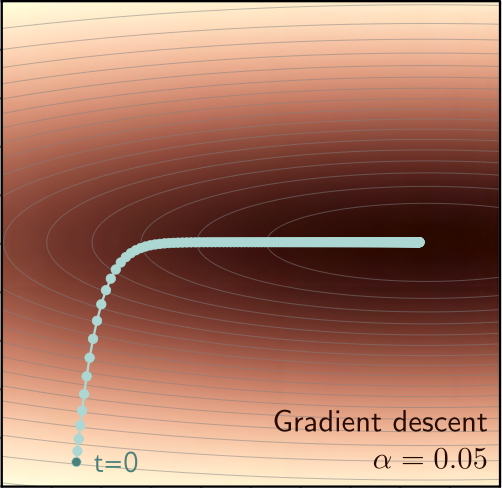
\includegraphics[width=0.4\textwidth]{Images/images_ch_2/grad_desc_1.png}
    }
    \hfill
    \subfloat[GD, $\eta=1{,}0$.\label{fig:gd_large_lr_grid}]{
        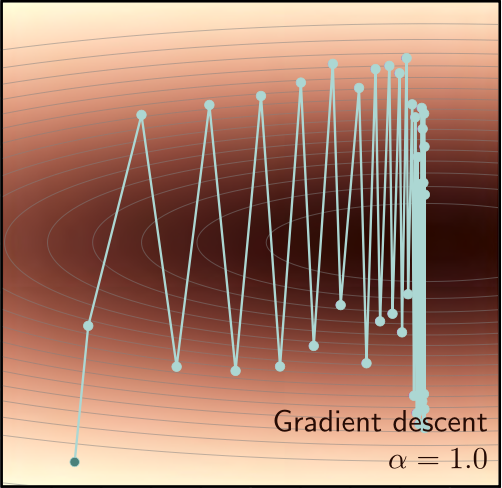
\includegraphics[width=0.4\textwidth]{Images/images_ch_2/grad_desc_2.png}
    }\\[1ex]
    \subfloat[Normalized gradients.\label{fig:norm_grad_grid}]{
        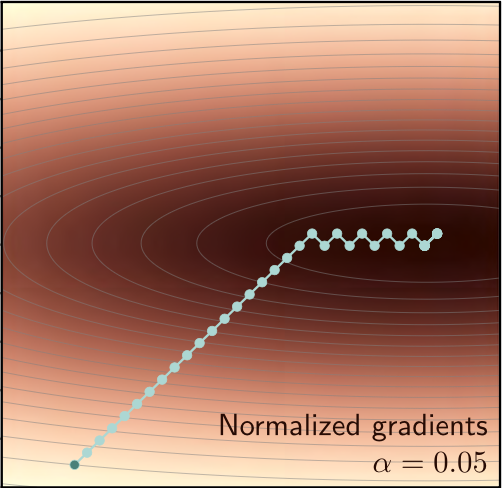
\includegraphics[width=0.4\textwidth]{Images/images_ch_2/norm_grad.png}
    }
    \hfill
    \subfloat[Adam.\label{fig:adam_grid}]{
        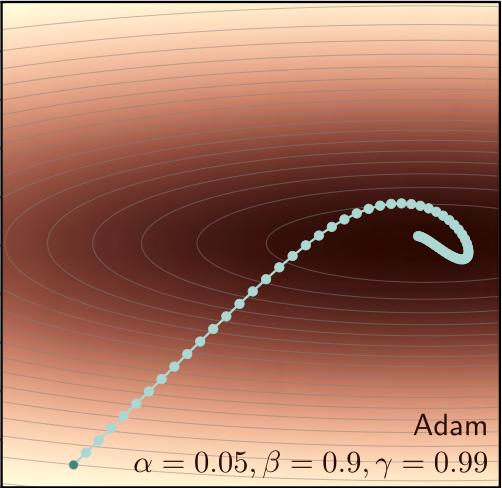
\includegraphics[width=0.4\textwidth]{Images/images_ch_2/adam.png}
    }
    \caption{Optimizer trajectories on an elongated bowl-shaped loss surface~\cite{prince2023understanding}.}
    \label{fig:optimizers_grid}
\end{figure}
